\documentclass[12pt]{article}

\usepackage{graphicx}
\usepackage[utf8]{inputenc}
\usepackage[english,russian]{babel}
\usepackage[pdftex,unicode]{hyperref}
\usepackage[margin=15mm,left=2cm]{geometry}
\usepackage{indentfirst}
\usepackage{amsbib}

\sloppy
\clubpenalty=999
\widowpenalty=9999

% This is all for formatting and making the Table of Contents according to 
% spec. Don't play with it.
\makeatletter
\renewcommand\l@section[2]{%
    \ifnum \c@tocdepth >\z@
        \addpenalty\@secpenalty
        \addvspace{1.0em \@plus\p@}%
        \setlength\@tempdima{1.5em}%
        \begingroup
        \parindent \z@ \rightskip \@pnumwidth
        \parfillskip -\@pnumwidth
        \leavevmode \bfseries
        \advance\leftskip\@tempdima
        \hskip -\leftskip
#1\nobreak\ 
        \leaders\hbox{$\m@th\mkern \@dotsep mu\hbox{.}\mkern \@dotsep mu$}
    \hfil \nobreak\hb@xt@\@pnumwidth{\hss #2}\par
        \endgroup
    \fi}
\makeatother

\title{Критерий планарности для класса предикатных схем}
\author{Василевская И.\,Ю.}
\date{\today}

\begin{document}
    \begin{titlepage}
        \begin{center}
            Московский Государственный Университет им. Ломоносова\\
            Факультет Вычислительной Математики и Кибернетики\\
            Кафедра Математической Кибернетики\\
            магистратура, отделение <<МММ СБИС>>\\[6cm]

            \large {Василевская Инесса Юрьевна}\\
            \LARGE \textbf {Верхние оценки одного параметра для класса предикатных схем}\\[0.8cm]
            \large \emph {Курсовая работа}\\[5.0cm]

            \begin{flushright}
                \large
                \begin{minipage}{0.40\textwidth}
                    \begin{flushleft}
                        \emph{Научный руководитель:}\\к.ф.м.н М.\,С.~Шуплецов
                    \end{flushleft}
                \end{minipage}
            \end{flushright}

            \vfill
            Москва\\
			2012
        \end{center}
    \end{titlepage}

\setcounter{page}{2}

\section{Введение}
\label{beginning}
В ряде работ (\cite{Shu09}, \cite{Shu11}) рассматривается задача синтеза для специального класса дискретных управляющих систем ~--
класса предикатных схем, который обобщает некоторые традиционные классы схем. Данные схемы строятся из предикатных элементов
и обладают рядом отличий от схем из других классов (например, направление протекания сигналов не является фиксированным).
Указанные выше работы в основном посвящены исследованию асимптотики функции Шеннона в классе предикатных схем,
 получению асимптотических оценок высокой степени точности и вопросам моделирования предикатными схемами схем из традиционных классов.

В силу особенностей класса предикатных схем, при его рассмотрении могут возникать вопросы,
нетипичные для традиционных классов. Так, к примеру, довольно любопытен вопрос функционирования предикатных схем с точки зрения оценки времени, которое нужно затратить для
вычисления конкретной схемы. 
В данной работе в качестве меры <<быстрой вычислимости>>\footnote{в англоязычной литературе употребляется термин tracktability}
 был выбран так называемый параметр \textit{ширины декомпозиции}~-- максимального числа вершин в узле дерева, 
которое можно оптимально построить по заданной предикатной схеме. Во многих работах (например, \cite{CSP10}, \cite{Gott10}, \cite{Prosc89}) было 
показано, что задачи, которые можно переформулировать в терминах Constraint Satisfaction Problem, быстро вычислимы, если ширина декомпозиции графа ограничений 
(constraint graph) ограничена сверху константой. 
Так как задача функционирования предикатных схем естественным образом представляется как задача CSP с булевыми ограничениями,
 вопрос <<быстрой вычислимости>> заданного предиката в конкретном базисе сводится к нахождению такого способа синтеза, 
 при котором результирующая схема будут иметь ограниченный параметр ширины декомпозиции
\footnote
{В англоязычных источниках известного как treewidth. В силу отсутствия общепринятого перевода, автор вводит 
понятие <<ширины декомпозиции>>}.

\section{Основные определения}
Ниже приведены формальные определения используемых в работе понятий.

\subsection{Предикатные схемы}

В настоящей работе определение предикатных схем будет дано по аналогии с \cite{Shu11}.

\textbf{Опредение}.
\textit{Схемой из предикатных элементов} или \textit{предикатной схемой в базисе $\Pi$} назовем помеченный
неориентированный двудольный граф следующей структуры:

\begin{itemize}
\item каждая вершина из первой доли помечена некоторым множеством символов из алфавита X и/или 
множеством символов из алфавита Y. 
Алфавит $X$ соответствует \textit{входным} переменным предиката, а $Y$ ~-- его внутренним переменным, 
т.е. переменным, возникающим непосредственно в процессе вычисления; 

\item каждая вершина второй доли помечена некоторым символом $\pi_i$ из множества $\Pi$ и 
соединена $k$ ребрами, пронумерованными числами $1, ..., k$, с вершинами из первой доли.
\end{itemize}

Вершины из первой доли будем называть \textit{узлами} схемы, а вершины из второй доли ~-- её \textit{предикатными элементами}. 
Узлы схемы, соединенные ребрами с предикатным элементом, будем называть полюсами этого элемента, 
а узлы, соответствующие входным переменным, ~-- полюсами схемы.
При этом считается, что узел является $j$-м полюсом предикатного элемента и соответствует 
его $j$-ой переменной, если соединяющее их ребро имеет номер $j$. Полюс схемы, которому приписано 
более одной входной переменной, называется кратным полюсом этой схемы. 

Будем считать элементарной такую предикатную схему, которая состоит либо из изолированной полюсной вершины, 
либо только из одного предикатного элемента $\pi_i$, $1 < i < k$, где $k$ ~-- число полюсов указанного элемента.

В тех случаях, когда это не вызывает разночтений, 
не будем различать узел схемы и переменную, 
символ которой приписан данной вершине, а также предикатный элемент и сам предикат, отвечающий этому элементу. 
Также, для удобства, в некоторых случаях будем использовать упрощенное описание предикатной схемы, 
опуская пометки дуг и некоторых внутренних вершин. 

\subsection{Функционирование предикатных схем}
\label{func}
Функционирование предикатного элемента с $k$ полюсами задается его характеристической функцией от $k$ переменных, 
связанных с указанными полюсами, и определяется тем, что предикатный элемент находится в допустимом состоянии на тех и 
только тех наборах значений этих переменных, на которых данная функция равна 1. 

Предикатная схема $\Sigma$ находится в допустимом состоянии на заданном наборе значений её полюсных переменных тогда и только тогда, 
когда существует такой набор значений внутренних переменных схемы, на котором все предикатные элементы схемы находятся в допустимых состояниях. 
Если же указанного набора значений внутренних переменных не существует, то считается, что схема находится в недопустимом состоянии на 
заданном наборе значений её полюсных переменных.

Предполагается, что предикатная схема $\Sigma$ реализует предикат $\pi$ от её полюсных переменных, если множество допустимых наборов $\pi$ 
совпадает с множеством тех наборов, на которых $\Sigma$ находится в допустимом состоянии. 
При этом схемы будем называть эквивалентными, если они реализуют равные предикаты. 
Отметим, что элементарная предикатная схема, состоящая из изолированной полюсной вершины, реализует тождественно истинный предикат.
 Будем считать также, что тождественно истинный (соответственно тождественно ложный)
 предикат реализуется любой предикатной схемой без входных полюсов, 
которая имеет непустое (соответственно пустое) множество допустимых состояний.

В общем случае граф предикатной схемы может содержать несколько компонент связности. 
В дальнейшем, будем считать, что схема не содержит компонент связности, 
которые не имеют полюсных узлов и для которых существует хотя бы один допустимый набор, так как такие компоненты не влияют на функционирование схемы.

Суперпозицией двух предикатных схем, не имеющих общих вершин и пометок, 
будем называть их объединение с возможным отождествлением группы полюсов этих схем, 
которое сопровождается приписыванием новой (``объединенной'') вершине либо 
некоторого подмножества переменных данной группы, либо ``новой'' внутренней переменной.
 При этом частными случаями суперпозиции являются следующие операции:
\begin{itemize}
\item переименование полюсной переменной схемы

\item введение фиктивной полюсной переменной схемы

\item проекция или снятие полюсной переменной схемы

\item отождествление двух полюсных переменных схемы
\end{itemize}

\subsection{Шефферов базис}

\textbf{Определение} ФАЛ
$f (x_1, \ldots, x_n)$ от $n$ переменных сохраняет предикат $ (x_1, \ldots, x_m)$ от $m$
переменных тогда и только тогда, когда для любых $n$ допустимых наборов $\alpha^i = (\alpha_1^i, \ldots, \alpha_n^i), 
i = 1, \ldots, n$ значений переменных предиката $\pi$ набор
значений $f((\alpha_1^1, \ldots, \alpha_1^n), \ldots, )(\alpha_m^1, \ldots, \alpha_m^n)$
тоже является допустимым для предиката $\pi$.

По аналогии с \cite{Shu11} определим следующие классы:
\begin{itemize}
    \item{$T_0$}~-- множество всех предикатов, сохраняющих константную ФАЛ 0.
    \item{$T_1$}~-- множество всех предикатов, сохраняющих константную ФАЛ 1.
    \item{S}~-- множество всех предикатов, сохраняющих ФАЛ $\bar{x}$.
    \item{K}~-- множество всех предикатов, сохраняющих все конъюнкции от двух и более переменных.
    \item{D}~-- множество всех предикатов, сохраняющих все дизъюнкции от двух и более переменных.
    \item{SM}~-- множество всех предикатов, сохраняющих все монотонные самодвойственные ФАЛ.
    \item{SL}~-- множество всех предикатов, сохраняющих все монотонные линейные ФАЛ.
\end{itemize}

\textbf{Теорема (Критерий полноты для предикатных схем)}. Система из $B$ предикатов является полной $\iff$
она не лежит целиком ни в одном из 7 предполных классов: $T_0, T_1, SM, SL, S, K, D$. \cite{Shu11} 

\textbf{Замечание} Если предикат $\pi$ принадлежит какому-либо предполному классу, применением 
операций горизонтальной (PROJECT)
и вертикальной (SELECT) выборки, перестановки переменных, отождествления входов (JOIN) и
взятия отрицания\footnote{Несмотря на то, что операция взятия отрицания не является базовой, согласно \S \ref{func},
в данной работе будут рассматриваться полные базисы, содержащие $\pi \notin K$, из которого предикат
$\bar{x}$((01), (10)) получается очевидным образом, поэтому будем считать эту операцию таковой}
одной или нескольких переменных $\pi$, получим
предикат $\pi_1$, принадлежащий тому же предполному классу.


Перебором можно убедиться, что множество всех шефферовых предикатов от не более чем трех переменных\footnote{
заметим, что в силу принадлежности всех предикатов двух переменных классу SM, шефферов предикат не может зависеть
менее чем от 3 переменных}, 
разбивается на три класса эквивалентности относительно операции
перестановки переменных и взятия отрицания одной или нескольких переменных. 

\begin{figure}[htb]
\centering
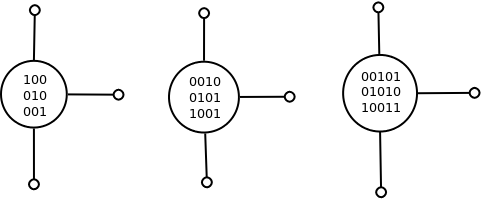
\includegraphics[width=0.5\textwidth]{scheff3.png}
\caption{Шефферовы предикаты от 3 переменных}
\label{fig:sheff}
\end{figure}


\subsection{Планарность}
\textbf{Определение.} 
Предикатная схема, которую можно уложить на плоскости без пересечений таким образом, что
все полюса предикатов лежат на внешней границе, называется планарной. 

\textbf{Определение.} Базис называется планарным, если в нем можно реализовать любой предикат планарной схемой.

Заметим, что операции JOIN2 (отождествление не более чем по двум переменным), PROJECT, SELECT и отрицание полюсов
сохраняют планарность. 

\textbf{Утверждение 1.} Шефферовы базисы на рис. \ref{fig:sheff} являются планарными.

В базисе $((001), (010), (100))$ \label{basis} можно планарной схемой реализовать предикат 
$((001), (010), (100), (111)) (\bar{\oplus})$. Замещая каждое реберное пересечение в схеме на 
3 предиката ($\bar{\oplus}$) по схеме \ref{fig:xor}, получаем планарную реализацию требуемого предиката
в базисе \ref{basis}.

Базис $((001), (010), (100), (011))$ сводится к базису \ref{basis} как показано на рисунке 
\ref{fig:scheff3_4}\footnote{Белыми кружками помечены полюса предиката}.
Базис $((001), (010), (100), (011), (101))$ сводится к базису \ref{basis} как показано на рисунке \ref{fig:scheff3_5}. 

\begin{figure}[htb]
\centering
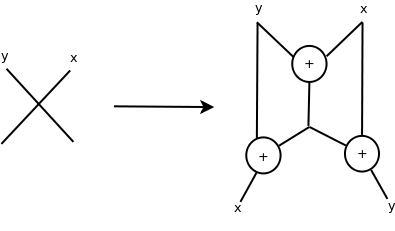
\includegraphics[width=0.5\textwidth]{intersection.png}
\caption{Получение планарной схемы}
\label{fig:xor}
\end{figure}


\begin{figure}[htb]
\centering
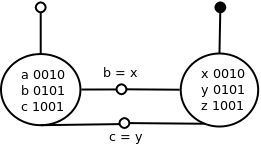
\includegraphics[width=0.4\textwidth]{scheff4.png}
\caption{Сведение к \ref{basis}}
\label{fig:scheff3_4}
\end{figure}


\begin{figure}[htb]
\centering
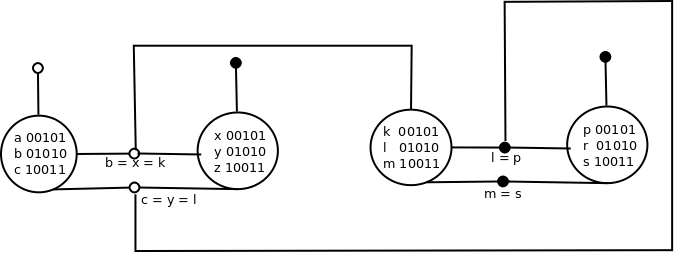
\includegraphics[width=0.7\textwidth]{scheff5.png}
\caption{Сведение к \ref{basis}}
\label{fig:scheff3_5}
\end{figure}

%\label{lemma1}
%\textbf{Утверждение.} Если $\pi$ сохраняет $f$ и $g$, то $\pi$ сохраняет композицию $f\circ g$.

\textbf{Лемма} Если $\pi \in P$, где $P$ ~-- предполный класс, $P \neq SM$, то, применяя операцию NEGATE,
можно получить $pi \notin P$. Например, $P = K$.
Однако, если $P = SM, \pi \in P или \pi \notin P$, операция NEGATE не изменяет принадлежность $\pi$ классу SM.

\textbf{Лемма} Система из $\pi_1 \notin SM, \pi_2 \in S$ полна.

\label{lemma_sm}
\textbf{Лемма} Рассмотрим $\pi \notin SM$ такой, что, предикат $\pi_1$, полученный вычеркиванием любой переменной, $\in SM$.
Пусть $\beta = (\beta_1, \dots, \beta_k)$~-- набор, $\notin \pi$, полученный в результате применения какой-то несамодвойственной функции.
Заметим, что $\beta \neq \forall \alpha \in \pi$. Однако, для соблюдения верхнего условия, $\pi$ должен содержать наборы 
$(\bar{\beta_1}, \beta_2, \dots, \beta_k), (\beta_1, \bar{\beta_2}, \dots, \beta_k), \dots, (\beta_1, \beta_2, \dots, \bar{\beta_k})$.
Нетрудно видеть, что эти наборы представляют собой обобщенный Шефферов предикат. 

Получаем следующее утверждение: 

\textbf{Утверждение} Если $\pi \notin SM$, то, применяя операцию PROJECT, можно получить минимальный предикат $\pi_1 \notin SM$, 
подмножество наборов которого будет обязательно составлять обобщенный Шефферов предикат.

Таким образом, для случая трех переменных, все несамодвойственные предикаты разбиваются на несколько классов эквивалентности 
(относительно операции PROJECT и перестановки переменных): 
\begin{itemize}
\item{Шефферов предикат из 3 наборов ($Sch_3$)}
\item{$Sch_3$ + 1 набор}
Заметим, что случай $Sch_3$ + (1111) не требует дополнительных преобразований и сведений, так как имеем планарную реализацию
$\oplus$, необходимую для планарного сведения по схеме \ref{fig:xor}
\item{$Sch_3$ + 2 набора}
\item{$Sch_3$ + 3 набора}
\item{$Sch_3$ + 4 набора}
\end{itemize}

Каждый из этих классов применением операций, не меняющих планарность схемы (SELECT, PROJECT, JOIN2, NEGATE), сводится к одному из 3
планарных Шефферовых базисов.

\textbf{Алгоритм для случая 3 переменных}
\begin{itemize}
\item{Получаем $\pi \in S$}
\item{Выделяем из полного базиса $\pi \notin SM$, сводим $\pi$ к предикатам из одного из 4 классов эквивалентности}
\item{По известным правилам получаем планарную схему}
\end{itemize}

\subsubsection{Случай $n > 3$}
В лемме \ref{lemma_sm} было показано, что множество наборов всякого минимального $\pi \notin SM$ содержит обобщенный
Шефферов предикат размерности $k$.

Покажем, что в случае, если базис $B$ содержит $\pi \notin SM$, $\pi$ зависит от более чем 3 переменных, существует планарная
сводимость $B$ к одному из трех планарных Шефферовых базисов (от 3 переменных).

\begin{itemize}
\item Шефферов предикат $Sch_4$ сводится к $Sch_3$ как показано на рисунке \ref{fig:4to3}
\begin{figure}[htb]
\centering
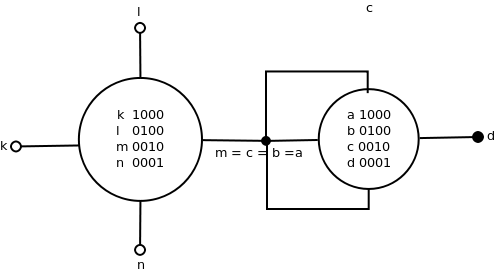
\includegraphics[width=0.6\textwidth]{4to3.png}
\caption{Сведение $Sch_4$ к $Sch_3$ \ref{basis}}
\label{fig:4to3}
\end{figure}

\item $Sch_4$ + 1 набор сводится к $Sch_4$ применением операции JOIN2 и PROJECT к предикату $Sch_4$ и предикату, 
полученному из $Sch_4$ перестановкой переменных. 
\begin{figure}[htb]
\centering
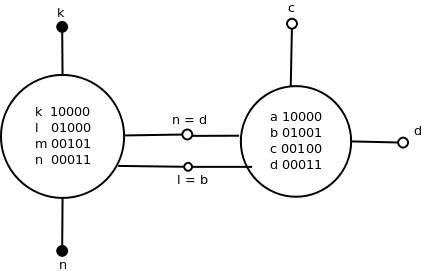
\includegraphics[width=0.6\textwidth]{4_1to4.png}
\caption{Сведение $Sch_4$ c одним набором к $Sch_4$ \ref{basis}}
\label{fig:4_1to4}
\end{figure}

\item $Sch_4$ + 2 набора сводится к $Sch_4$ + 1 набор применением JOIN2 и PROJECT
\begin{figure}[htb]
\centering
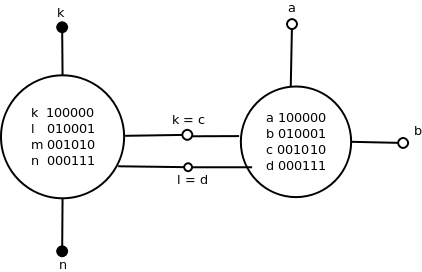
\includegraphics[width=0.6\textwidth]{4_2to4_1.png}
\caption{Сведение $Sch_4$ c одним набором к $Sch_4$ \ref{basis}}
\label{fig:4_2to4_1}
\end{figure}

$\ldots$

\end{itemize}

Нетрудно видеть, что, за счет симметричности Шефферова предиката, и несимметричности ``дополнительных'' наборов, можно 
перестановкой переменных одного из предикатов и последующим применением операции JOIN2 на ((00), (01), (10)), сводить 
каждый следующий случай $Sch_4 + k$ к предыдущему $Sch_4 + k-1$, исключая ``лишний'' набор.

Данный алгоритм не подходит, если добавляемые наборы симметричны\footnote{Нет возможности по аналогии
получить набор ((00), (01), (10))}: $Sch_4$ + (1111)
% Список цитируемой литературы
\clearpage
\addcontentsline{toc}{section}{Список цитируемой литературы}
\thebibliography{99}
\RBibitem{Shu09}
    \by М.~С.~Шуплецов
    \paper Оценки высокой степени точности для сложности предикатных схем в~некоторых базисах
    \inbook Физико-математические науки
    \serial Уч\"eн. зап. Казан. гос. ун-та. Сер. Физ.-матем. науки
    \yr 2009
    \vol 151
    \issue 2
    \pages 173--184
    \publ Изд-во Казанского ун-та
    \publaddr Казань
    \mathnet{http://mi.mathnet.ru/uzku760}

\bibitem{Shu11}Методы синтеза и оценки сложности схем, построенных из элементов предикатного типа, диссертация

\bibitem{CSP10} Handbook of Constraint Programming, ISBN 9780444527264; 2010 г.

\bibitem{Shaeffer78} Schaefer, Thomas J. (1978). 
``The Complexity of Satisfiability Problems''. STOC 1978. pp. 216–226. doi:10.1145/800133.804350.

\bibitem{Zarank54} Zarankiewicz, K. "On a Problem of P. Turán Concerning Graphs." Fund. Math. 41, 137-145, 1954. 

\bibitem{Prosc89} Arnborg, S.; Proskurowski, A. (1989), 
``Linear time algorithms for NP-hard problems restricted to partial k-trees'',
Discrete Applied Mathematics 23 (1): 11–24, doi:10.1016/0166-218X(89)90031-0.

\bibitem{Gott10} 
Georg Gottlob, Reinhard Pichler, and Fang Wei. 2010. Bounded treewidth as a key to tractability of knowledge representation and reasoning. Artif. Intell. 174, 1 (January 2010), 105-132. DOI=10.1016/j.artint.2009.10.003 http://dx.doi.org/10.1016/j.artint.2009.10.003

\bibitem{Diestel00}
Diestel, Reinhard (2000), Graph Theory, Graduate Texts in Mathematics, 
173, Springer-Verlag, ISBN 0-387-98976-5.

\bibitem{Boedlander96}
H. L. Bodlaender, A linear-time algorithm for finding 
tree-decompositions of small
treewidth, SIAM J. Comput. 25 (1996), 1305–1317


\endthebibliography

\end{document}
